\documentclass{beamer}
\usetheme{Dresden}

\title{DOC2PPT: Automatic Presentation Slides Generation from Scientific Documents}
\author{Tsu-Jui Fu, William Yang Wang, Daniel McDuff, Yale Song}
\date{\today}

\begin{document}

\frame{\titlepage}

\begin{frame}{Abstract}
    This paper introduces DOC2PPT, a task for generating presentation slides from scientific documents that involves summarization, image retrieval, and organizing content for presentation. The authors propose a hierarchical sequence-to-sequence approach that outperforms strong baselines, with an accompanying dataset of approximately 6,000 document-slide pairs.
\end{frame}

\begin{frame}{Introduction}
    Creating presentations requires complex reasoning skills to summarize and visually arrange information, which raises the question of whether machines can replicate this process. The authors elaborate on the unique challenges in automated slide generation from documents, considering both textual and visual elements.
\end{frame}

\begin{frame}{Related Work}
    The authors provide an overview of relevant literature in vision-and-language modeling, document summarization, and multimodal summarization, highlighting that previous work does not adequately address the unique challenges posed by generating structured outputs, specifically presentation slides. They emphasize the novelty of the DOC2PPT task within this context.
\end{frame}

\begin{frame}{Approach}
    The DOC2PPT model involves reading a document, paraphrasing content for slides, and strategically determining object placement on each slide. The architecture includes a modular design with components for document reading, progress tracking, object placement, and paraphrasing.
\end{frame}

\begin{frame}{Model}
    The model employs a Document Reader that encodes the document's text and figures, a Progress Tracker that governs the hierarchical structure, and an Object Placer that determines slide content and layout. The Paraphraser reformulates text to be concise and suitable for presentation.
\end{frame}

\begin{frame}{Training}
    The authors establish a training methodology that balances structural and content similarity, ensuring that the generated slides closely follow the format and substance of the ground truth. Various components of loss are defined to assess the quality of selected content and layout.
\end{frame}

\begin{frame}{Inference}
    During inference, a multimodal projection head helps refine the generated slides by adding relevant figures and removing irrelevant ones based on a set threshold. This post-processing step enhances the final slide deck's informativeness.
\end{frame}

\begin{frame}{Dataset}
    The dataset includes 5,873 pairs of documents and slide decks sourced from various research communities, providing a comprehensive resource for training and evaluation. The authors outline the data collection and extraction processes ensuring robustness and reliability.
\end{frame}

\begin{frame}{Experiments}
    The authors propose new evaluation metrics specifically for slide generation, performing comprehensive assessments of their approach against various baselines. They also conduct human evaluations to gauge perceived slide quality.
\end{frame}

\begin{frame}{Results and Discussions}
    The results show that the hierarchical modeling employed in DOC2PPT outperforms flat models across various evaluation metrics. The authors also discuss the effectiveness of individual components in the architecture, such as paraphrasing and layout prediction.
\end{frame}

\begin{frame}{Conclusion}
    The authors highlight the significance of their work in advancing automatic slide generation, addressing multimodal challenges, and contributing a substantial dataset and evaluation metrics for the community. They anticipate that DOC2PPT will foster improvements in vision-and-language understanding.
\end{frame}

\begin{frame}{Extracted Figure}
    \centering
    \begin{figure}
        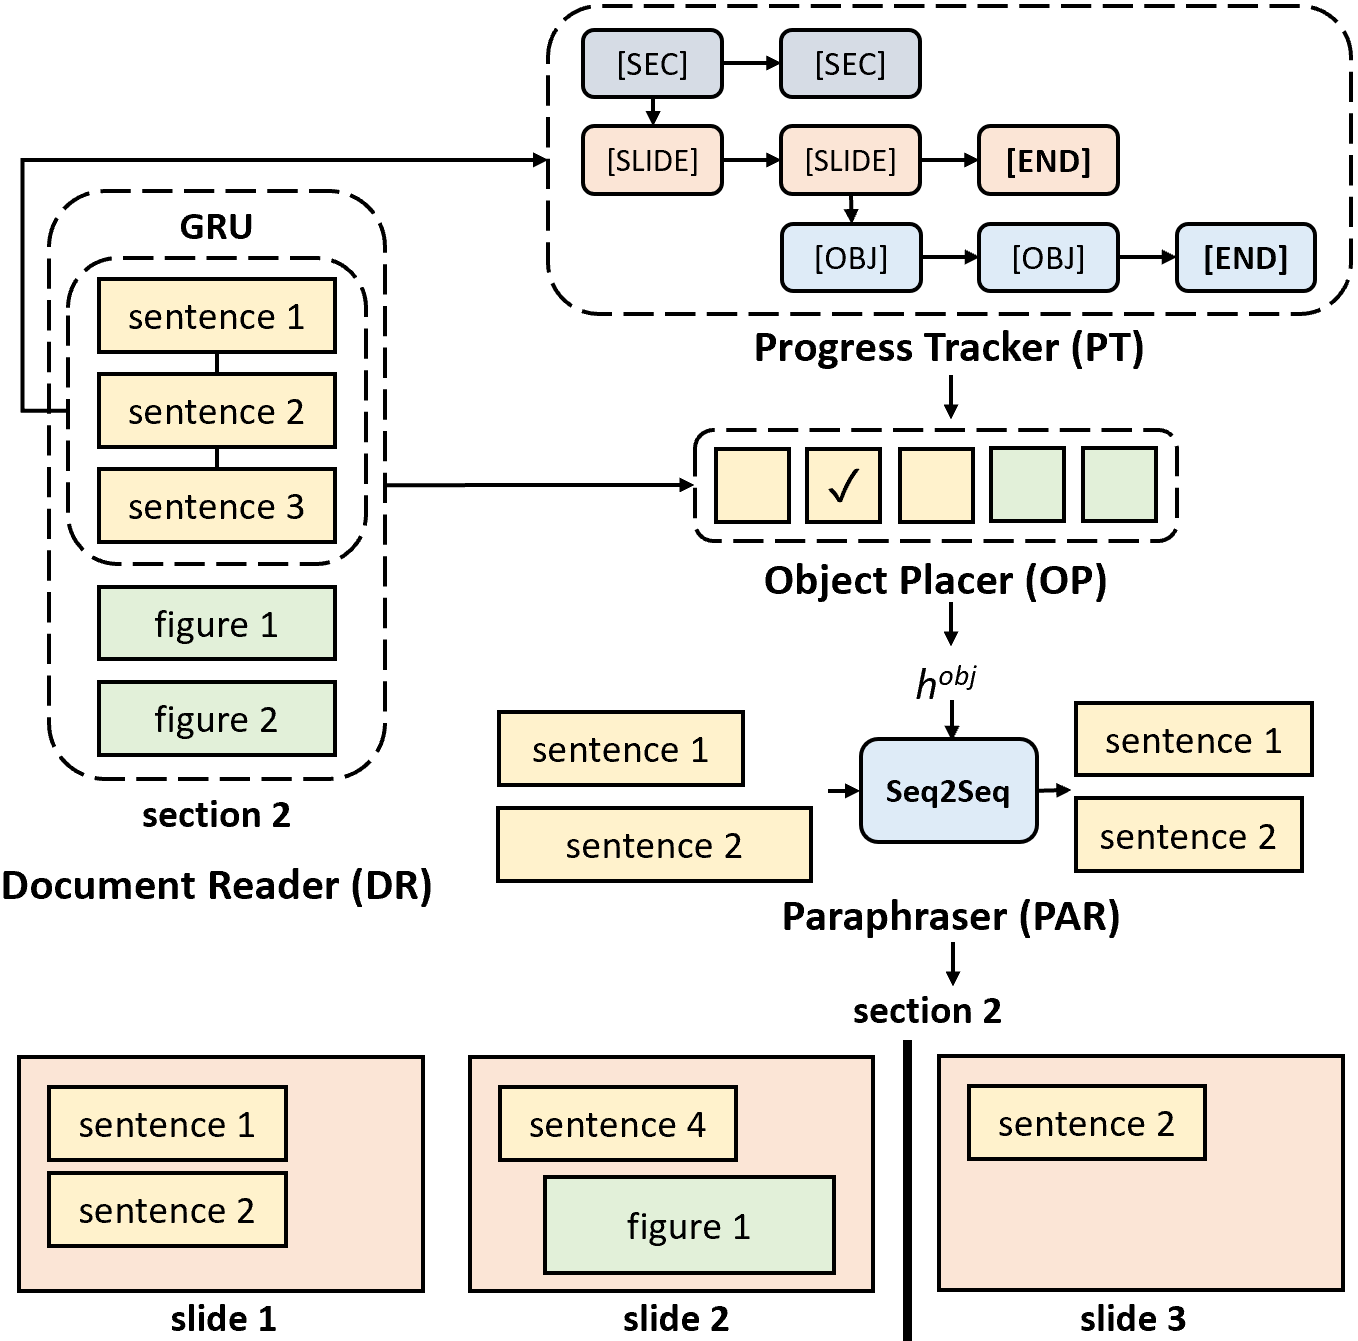
\includegraphics[width=0.8\textwidth]{extracted_images/figure_3_1.png}  % Relative path inside slides/
    \end{figure}
\end{frame}

\begin{frame}{Extracted Figure}
    \centering
    \begin{figure}
        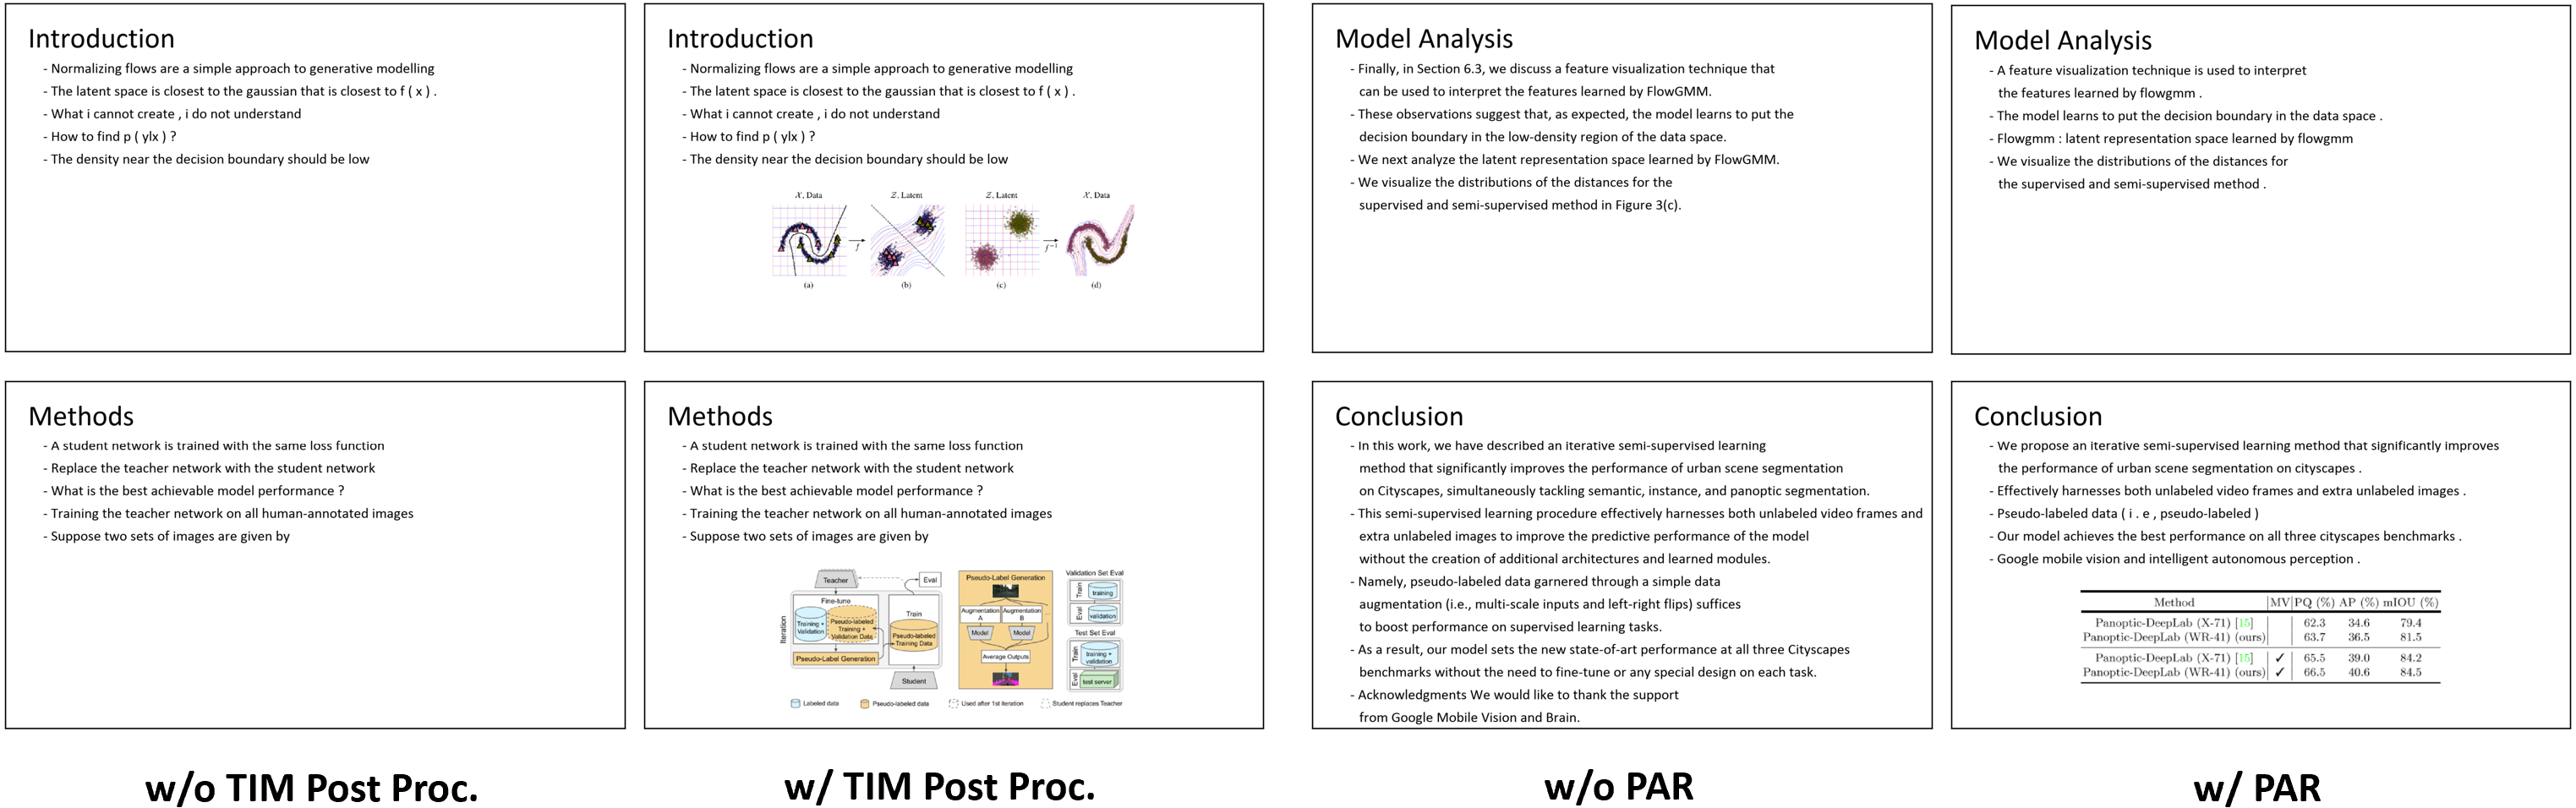
\includegraphics[width=0.8\textwidth]{extracted_images/figure_7_1.png}  % Relative path inside slides/
    \end{figure}
\end{frame}

\end{document}